\section{Evaluation} \label{sec:evaluation}

\todo{completely rework when settled on results story}

One simple heuristic value function that we can try is simply picking the action corresponding to the class presence variable $C_k$ with the highest probability.

We use one-vs-all deformable part-model classifiers on a HOG featurization of the image \cite{Felzenszwalb2010a}, with associated linear classification of the detections.

\begin{figure}[h!]
\centering
\subfloat[Occurence of a class with another]{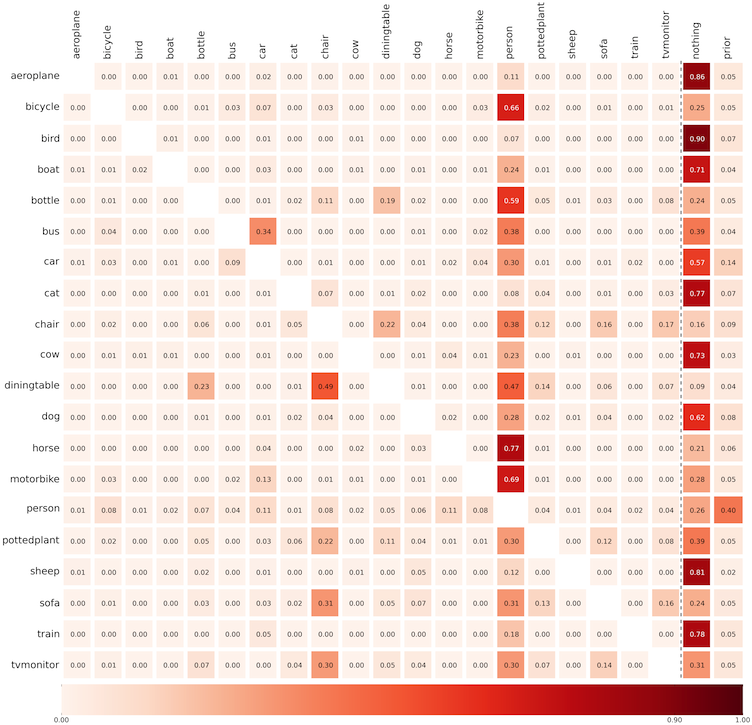
\includegraphics[]
    {../figures/full_pascal_trainval_stats/cooccur_trim.png}} \hfill
\subfloat[Occurence of a class with two others]{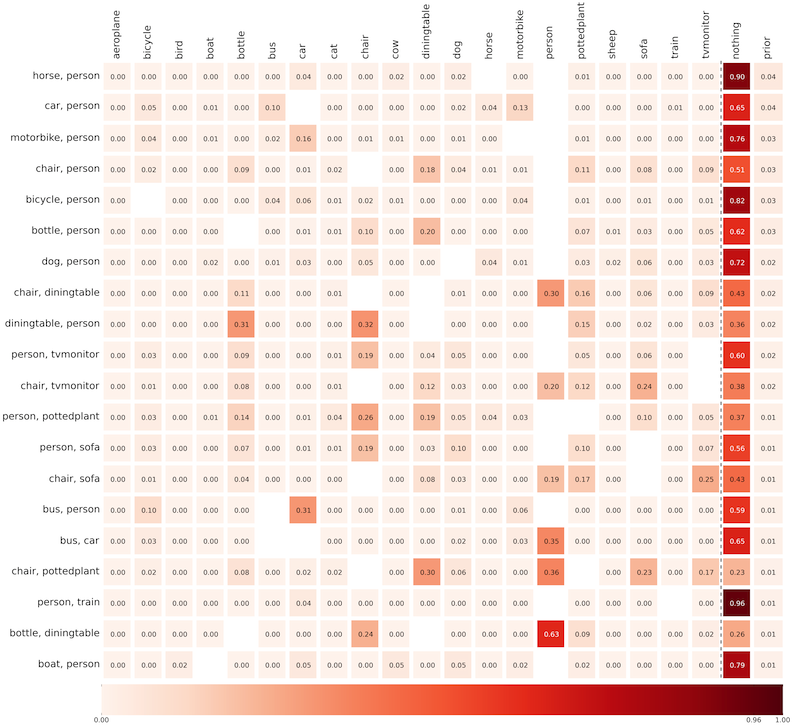
\includegraphics[]
    {../figures/full_pascal_trainval_stats/cooccur_second_order_trim.png}}
  \caption{
  Co-occurrence statistics on the training portion of the PASCAL VOC 2007 dataset.
  In the first plot, a (row,column) cell shows the probability that an image that contains an object of the row class also contains an object of the column class.
  Accordingly, in the second plot, the probability that an image containing objects of the two classes listed in the row also contains an object of the column class.
  }
  \label{fig:dataset_stats}
\end{figure}

To summarize \autoref{sec:}, we evaluate our system in the multi-class, multi-label detection regime.
We evaluate on a popular detection challenge task: the PASCAL VOC dataset \cite{pascal-voc-2010}.
As shown in \autoref{fig:dataset_stats}, the dataset exhibits a rather modest amount of class co-occurrence, which puts our model in a disadvantaged setting.
$60\%$ of the images in the training set have only one class; $30\%$ have two classes, $7\%$ have three classes, and almost none have more.

Using the 2007 version of the dataset, we train on the training and validation data and test on the test set.
We run our policies on all images in the test set, cutting off execution at $T_d$.

To evaluate performance at a given time, we gather all detections and the classification answers found to this point in all the recognition episodes.
As described before, we evaluate detection performance by averaging per-image performance in the multi-class regime.
We evaluate classification performance by pooling the ground truth across the dataset, in standard procedure.

We establish the baseline performance of our system by selecting actions randomly at each step.
The time setting for our evaluation is $T_s=0$, $T_d=20$ (in seconds).
As shown in Figure~\ref{fig:results_manual}, the random policy results in a roughly linear gain of performance vs. time.

To establish an upper bound on performance, we also plot the Oracle curve, obtained by re-ordering the actions with the hindsight of the results they produced.
Note that the curves turn downward in this setting: this is due to the different performance levels of the detectors: as the weaker detectors are inevitably run, they introduce more false positives and false negatives than true positives.

\begin{figure}[h!]
\centering
\subfloat[AP vs. Time curves]{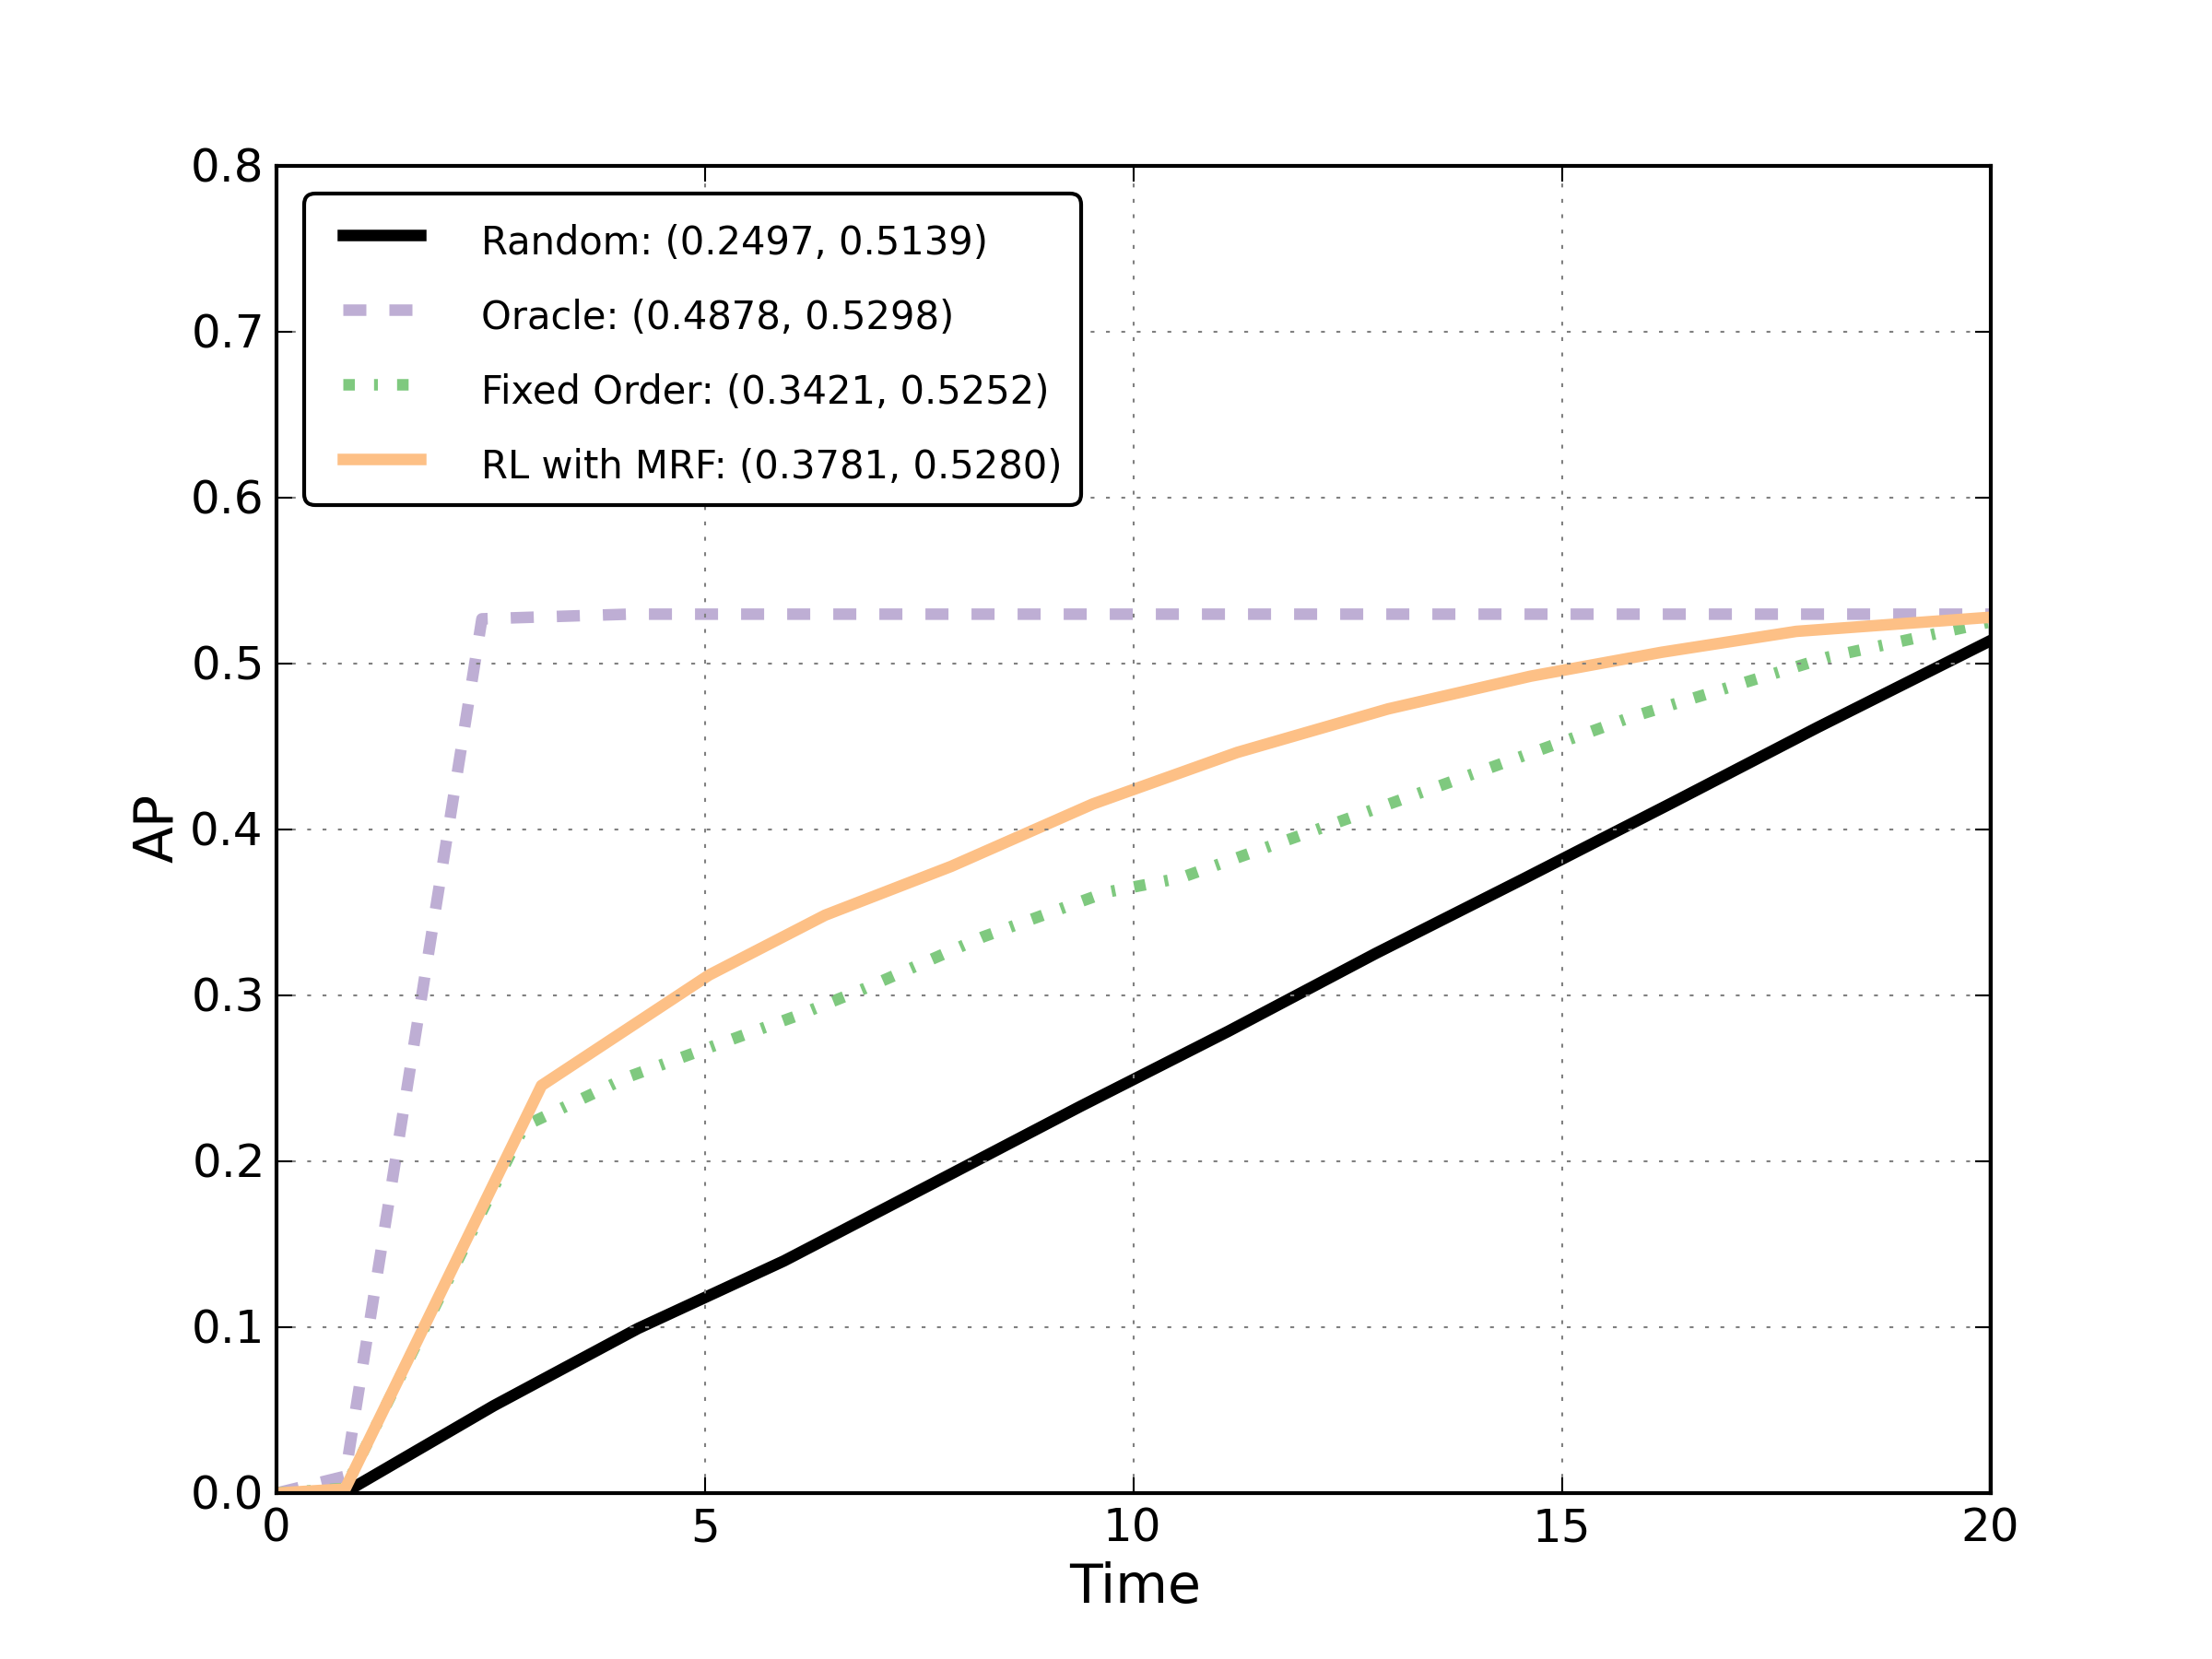
\includegraphics[width=0.47\linewidth]
    {../figures/final1.png}} \hfill
\subfloat[Execution traces of different policies]{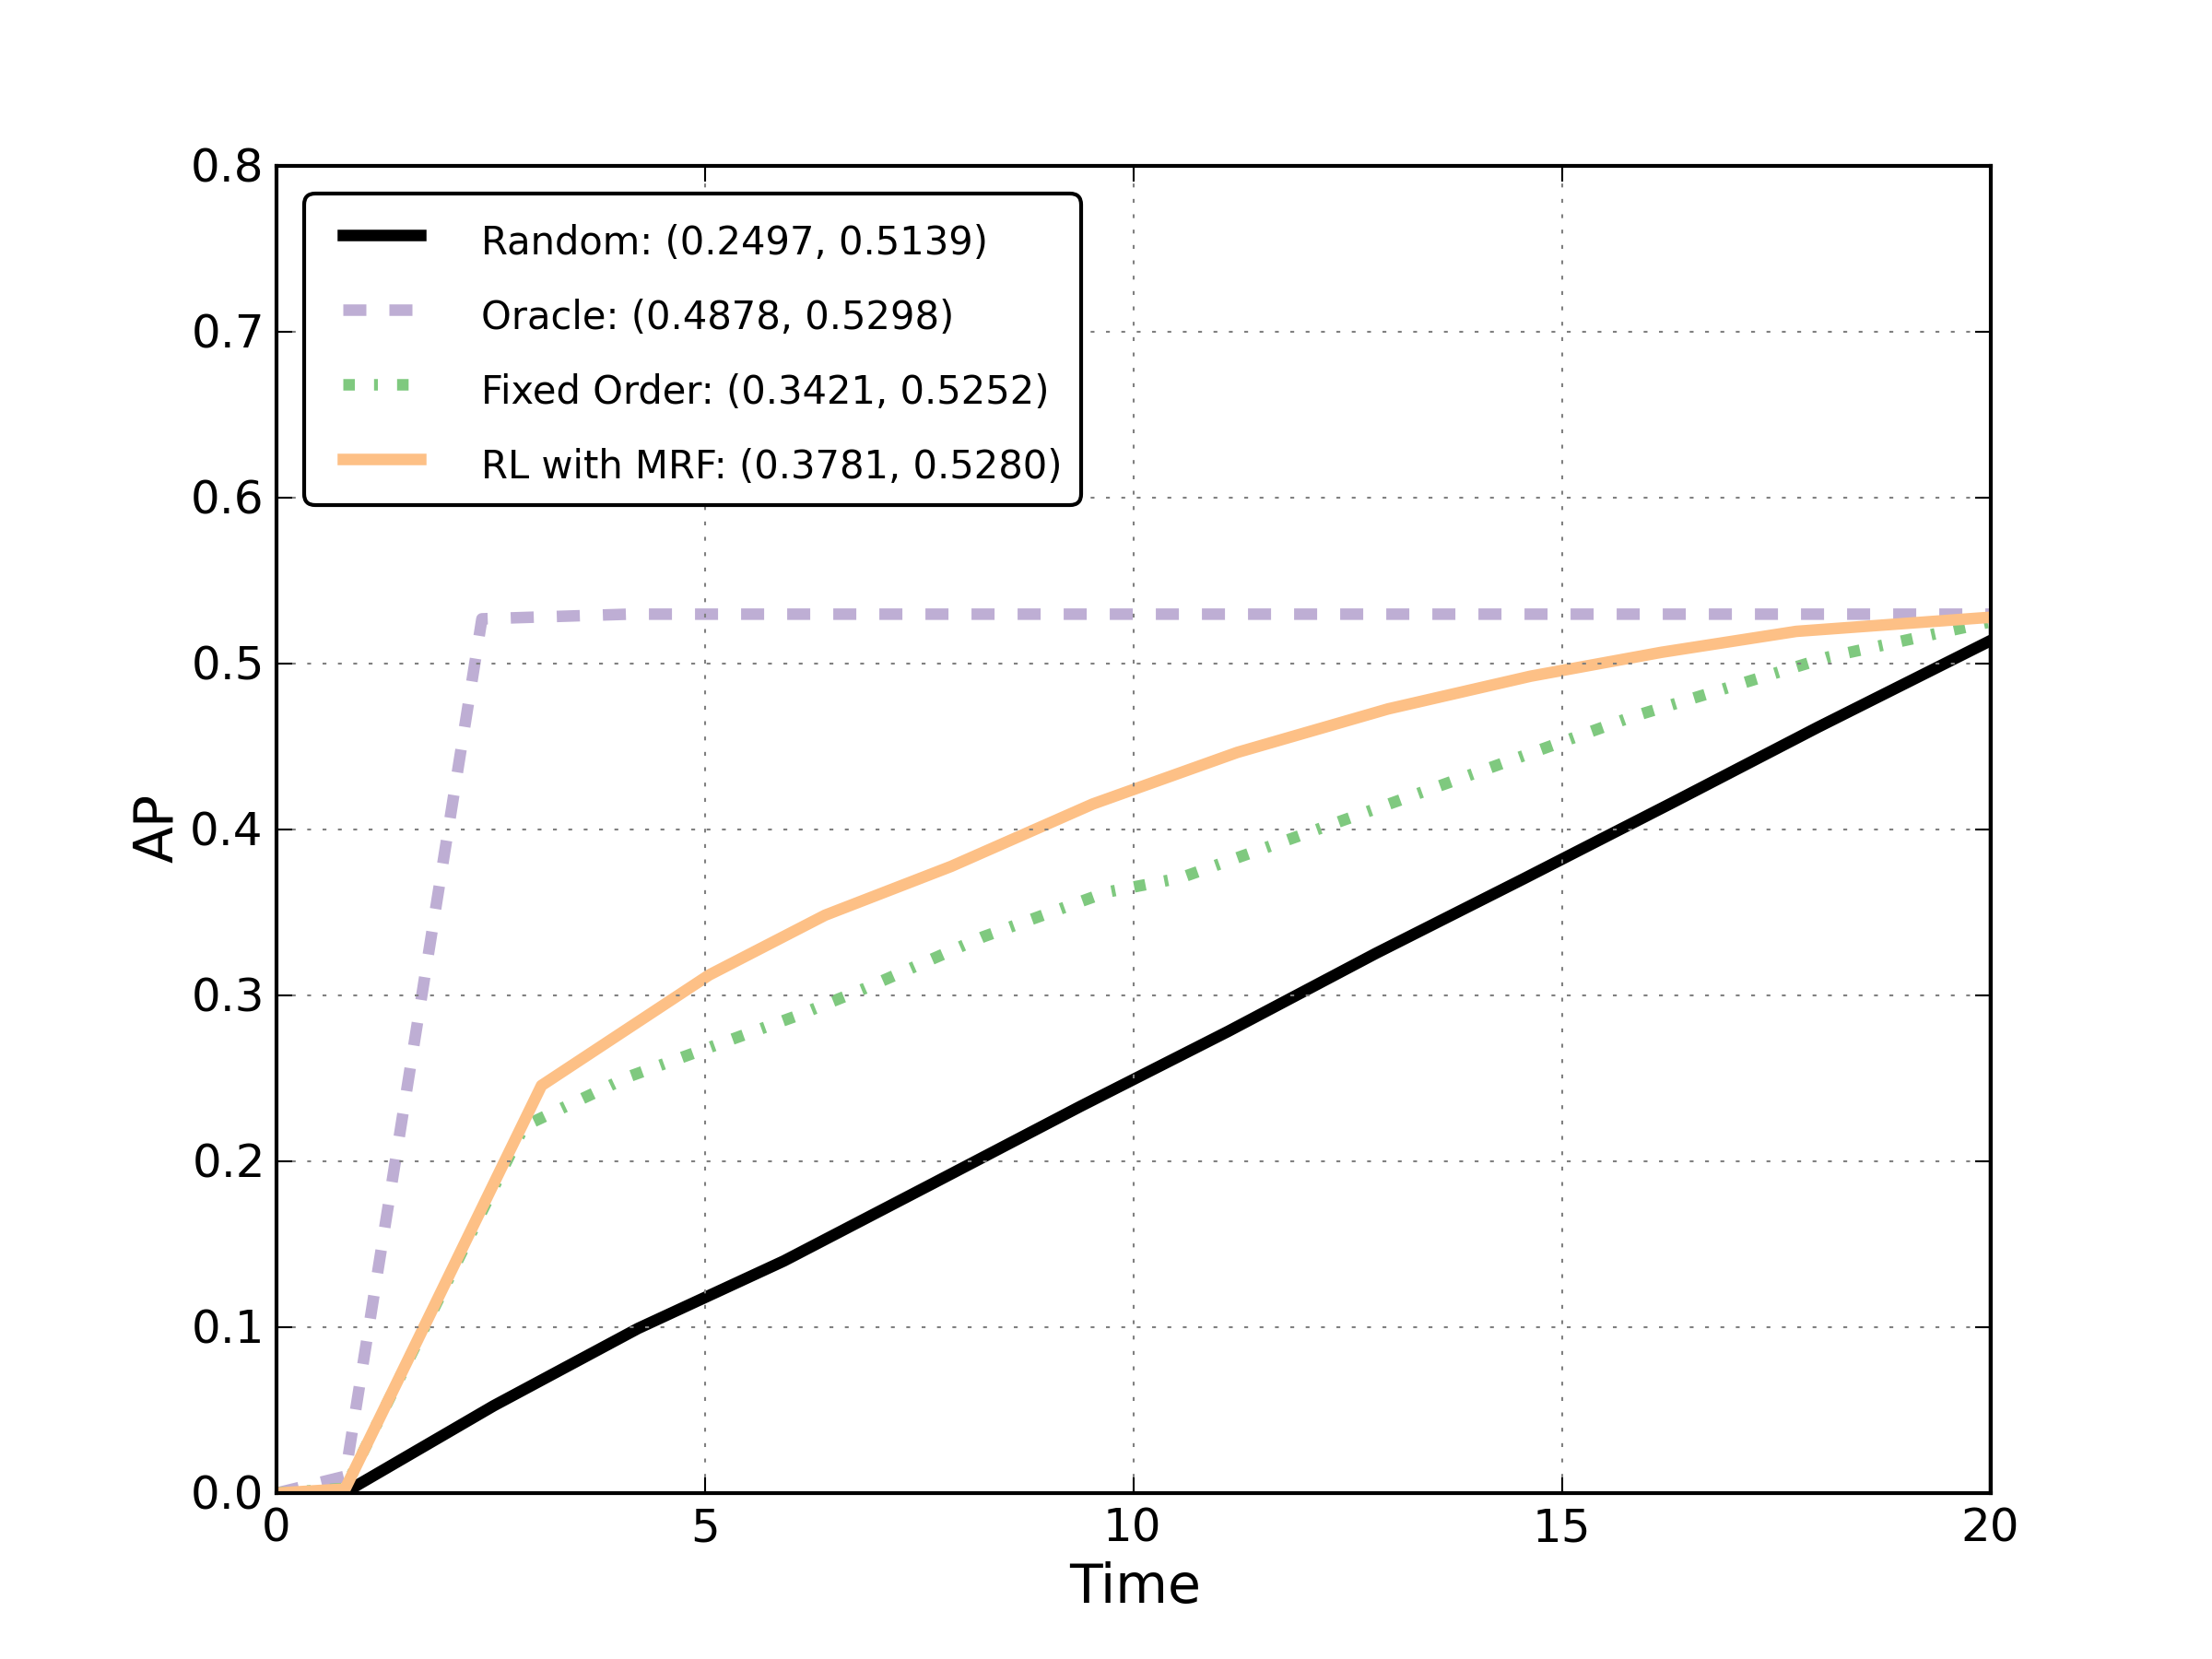
\includegraphics[draft,width=0.47\linewidth]
    {../figures/final1.png}}
  \label{fig:results1}
\end{figure}

\begin{table}[t]
\caption{Results}
\label{tab:results}
\begin{center}
\begin{tabular}{|l|l|l|l|l|l|}
\\ \hline \\
Bounds & Random & Fixed Order & RL w/ MRF & w/ GIST   & Oracle \\ \hline
(0,10) & 0.1191 & 0.2404      & 0.2664    & 0.2665    & 0.4638 \\ 
(0,20) & 0.2497 & 0.3421      & 0.3781    & 0.3824    & 0.4878 \\ 
(5,15) & 0      & 0           & 0         & 0         & 0      \\
\end{tabular}
\end{center}
\end{table}

Figure~\ref{fig:results1} also shows the performance of our policy with the heuristic value function and two inference models: the MRF model and a simple fixed-order model that follows the priors.
We can see that due to the dataset bias, the fixed-order policy performs well at first (the person class is disproportionately likely to be in the image), but is overtaken by the proper inference model as execution goes on.

A notable difference between the MRF inference model and the fixed-order model was in the weights learned: while the fixed-order model learned weights onto the bias feature only, the MRF inference model learned weights onto a mix of the entropy and probability features
